\chapter{Methodology}\label{chap2}
\thispagestyle{plain}

%This chapter provides a detailed description of the methodology. It is
%sometimes called Experimental Section. Depending on the subject it is a
%``synonym'', e.g., for Theoretical Section, Computational Methods, Model
%Description and Setup, Field Work, and so on. Hence, this chapter contains a
%description of \emph{what has been done} in order to address the scientific
%question raised in the chapter Introduction. However, it does \emph{not} contain
%the results! 


% ==== SECTION 1 ===============================================================
%\section{Experimental Set-up}\label{2sec:1}
%Depending on the topic of the science thesis, this chapter may contain a
%description of the experimental set-up, the field experiment,
%datasets, instruments, measurement procedures, analysis techniques, calibration
%and quality control, and other things. In case of a modeling study it may
%contain the formulation and derivation of model equations, the formulation of
%initial and boundary conditions, the data used to drive and validate the model,
%an overview of the model set-up (e.g., parameter set-up), modifications of the
%``original'' model code, a description of relevant parameterizations,
%a theoretical background needed for the interpretation of model results.


% ==== SECTION 2 ===============================================================
\section{Data Sets}\label{glathida}
This section gives an overview of the data used in the analysis done in this thesis. The basics data to run all the analysis have been the Glacier Thickness Database (GlaThiDa), the Randolph Glacier Inventory (RGI), and different digital elevation models (DEMs) which are dependent on the specific glacier. Depending on the region in fact some digital elevation models are a better fit to each glaciers as all of the freely available ones have missing data. ``The best'' digital elevation model has been automatically chosen by the Open Global Glacier Model (OGGM). Through most of the analysis SRTM v4 (\citet{SRTM}) which is a 90m grid resolution DEM has been used. Other DEM might have been used to link the GlaThiDa with RGI (see section \ref{GlaRGI})

\subsection{GlaThiDa}
The glacier Thickness Database (\citet{GlaThiDa2014}) is a set of data which attempts to put together all the available ice thickness measurements from glaciers and ice caps all around the globe. The database is composed of three different tables. The first one contains an overview of the database, the second one thickness data from maps or digital elevation models (DEM), and the third one, the one used in this thesis, contains the actual point measurements with the thickness data. The measurements were taken with different methods such as terrestrial and airborne radio-echo sounding, ground penetrating radar, direct drilling and other methods. The first database was released in 2014. In 2016 a second version 2.0 and its correction 2.1 were released, and in 2019 version 3.0 and 3.01 were finally released. All the analysis in this work have been done using version 2.1 as version 3.0 was released after a big part of the analysis was already done. According to the \href{https://github.com/ezwelty/glathida/blob/master/CHANGELOG.md}{change log} however most of the changes have been done to the structure of the data base. There were however some measurements additions to the database. The addition of some measurements for some glaciers in Switzerland in particular would be relevant for this thesis, given that most of the analysis done in this work has been conducted over the alpine glaciers. 
%Use subsections to structure your thesis. The first and second component of the
%momentum equation is shown in equation (\ref{2equ:1}) and (\ref{2equ:2}),
%respectively. Together with (\ref{2equ:3}) they form the set of shallow-water
%equations implemented in a numerical model.

\subsection{RGI}
The Randolph Glacier Inventory (RGI) (\citet{RGI2014}) is a global database of outlines of glaciers, excluding ice sheets. The inventory has been compiled from satellite imagery collected from 1999 onward. Most of the outlines don't express a specific picture in time of the glacier but are a compound of different images of each glacier due to images obstructions such as cloud covers or satellite orbits. The first version of this inventory was released in 2012 and the latest version, RGI Version 6.0 was released in 2017. In this latest release the database comprises more than 220,000 glacier outlines which are divided in 19 regions which cover all areas in the world with glaciers. This is the version used for all the analysis in this thesis. \todo{Add map of all the glaciers?}

\subsection{Linking GlaThiDa and RGI}\label{GlaRGI}
The GlaThiDa comes with a table containing the thickness measurements observations. This table comes with the thickness value of the observation, its latitude and longitude, and other variables such as the date of the observation, the name of the glacier, the thickness uncertainty and others. Aside from the measurements GPS coordinates and the thickness value, some fields like, the name of the glacier and the thickness uncertainty, are often left empty. This creates the problem of having to link each observation with a glacier in the RGI database. To do so a script has been created which determines whether an observation is located inside a glacier outline: the RGI database comes with closed outlines of the glaciers in geographic coordinates referenced to the WSG84 (also known as ESPG:4326) as shape-files. The python library \href{https://github.com/Toblerity/Shapely}{shapely} has been used to transform the observation Latitude and Longitude to the WSG84 projection system and to check whether each of these point was lying inside the glacier outlines (including the boundaries of the outline).
\todo{Add graphic of a glacier with the thickness points. I couldn't find a script with it so far.}

\subsection{Some statistics about GlaThiDa}
After linking the two databases it is interesting to learn about some statistics of the GlaThiDa. In order to create these statistics The Open Global Glacier Model (OGGM) (\citet{OGGM2019}, \href{https://github.com/OGGM/oggm}{Open Source Code}) has been used to add a digital elevation model to the glaciers in the RGI with thickness entries in the GlaThiDa (see \ref{GlaRGI}).

\subsubsection{Glaciers distribution and types}
There are 820370 entries (thickness measurements) in the GlaThiDa version 2.1. After assigning each of them to one of the 215,547 RGI glaciers 771 of those glaciers have thickness observations associated with them. This is 0.36\% of all the glaciers in th RGI. Out of the 820370 initial entries 27882, 3.4\% resulted outside of any glacier outlines defined in the RGI. Some reason for this could be: a slightly wrong GPS coordinate collected in the GlaThiDa measurement; observations taken outside of the glacier by mistake or intentionally, to make sure that all the glacier was covered; a different shape of the glacier at the moment when the observation was taken, compared to the moment when the RGI was compiled; a wrong assessment of the glacier shape in the RGI.
\begin{figure}\label{glathidamap} 
	\centering 
	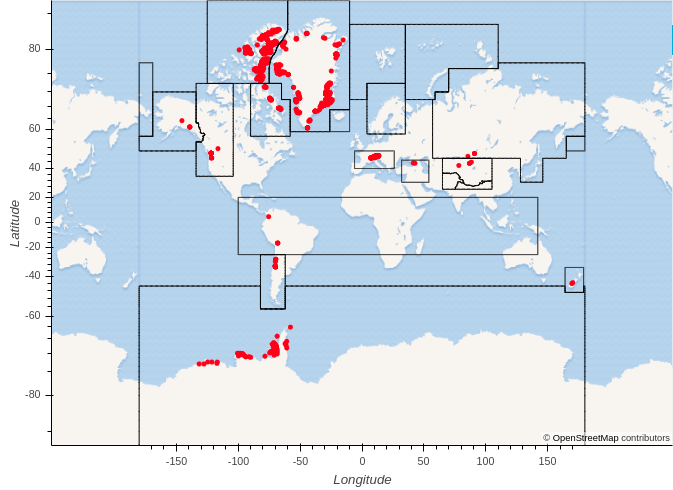
\includegraphics[width=1.0\textwidth]{./figures/GlaThiDa_map.png}
	\caption{Global map of the distribution of glaciers with thickness observations entries in the GlaThiDa database version 2.1. Black outlines are the RGI regions.}
\end{figure}

Most of the glaciers with thickness observation are in the Greenland Periphery region and in the Artic Canada North region. If we compare the glaciers with measurements with the number of glaciers present in each specific region though, we see that Arctic Canada North is the best represented region with around 5\% of the glaciers having at least one thickness measurement point. The region with most glaciers, Central Asia, has a very low number of glaciers represented in the GlaThiDa database. This is probably due to the difficulty in getting measurements for glaciers as such high altitudes at those present in the Himalaya.


\begin{figure}[!tp]
	\centering		  
	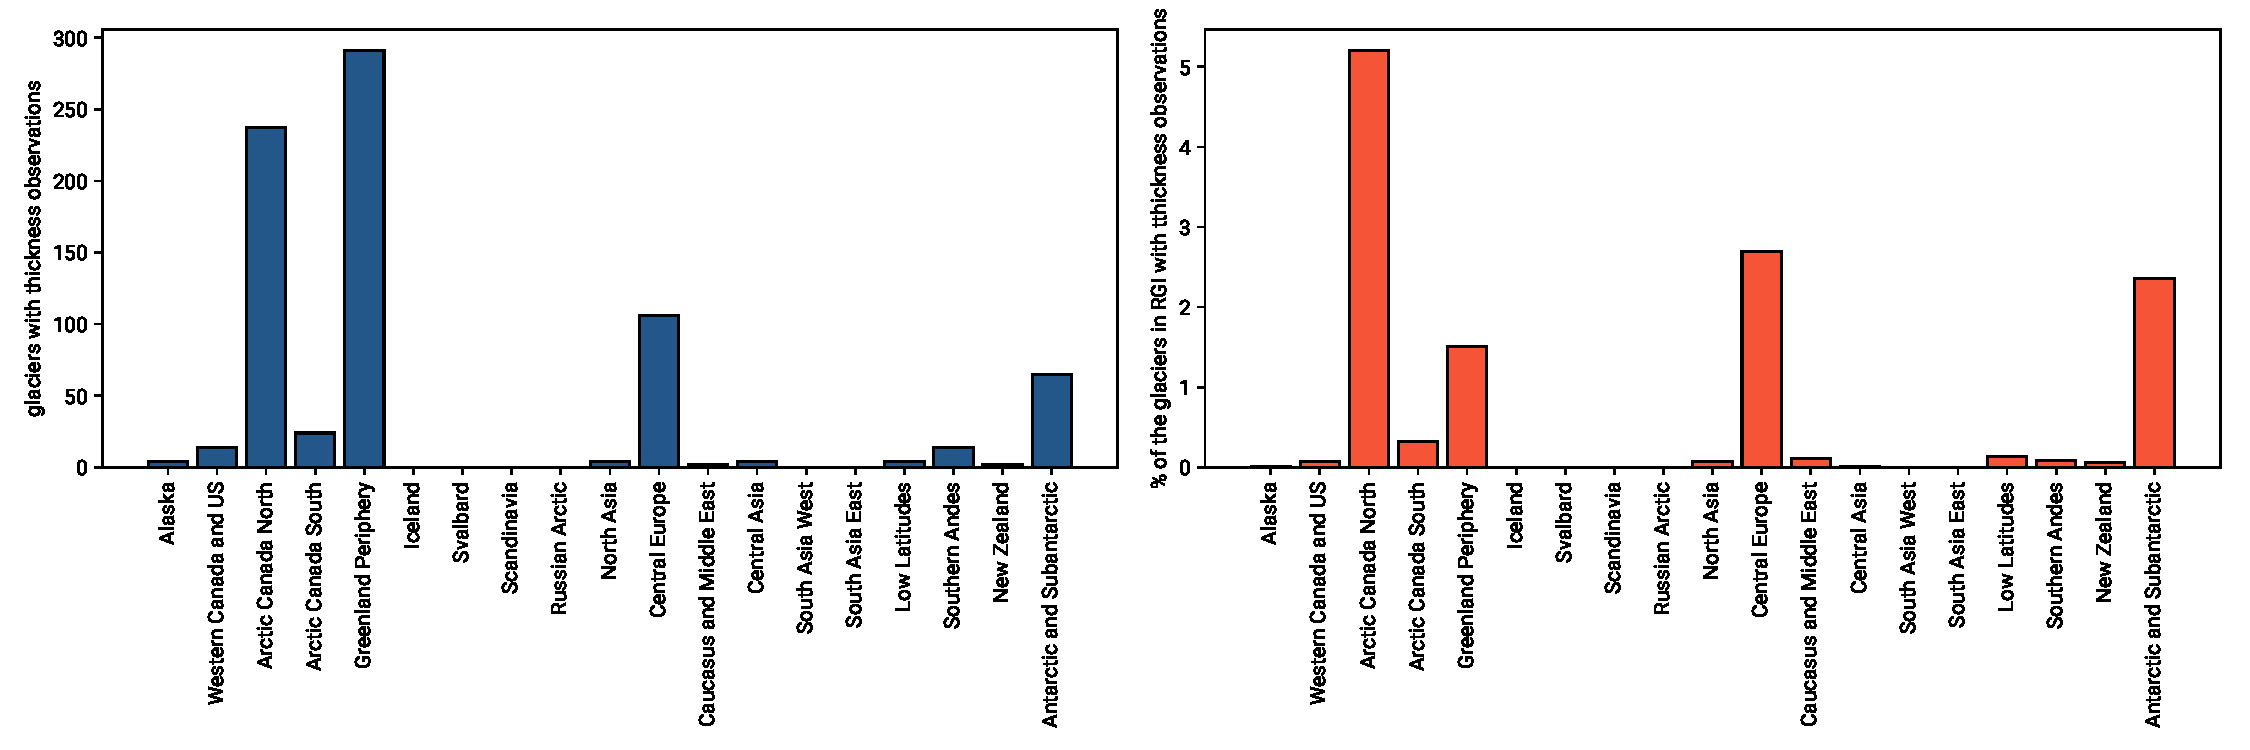
\includegraphics[width=1.\textwidth]{figures/Observations_per_region.pdf}
	\label{fig:glareg}
	\caption{On the left side the number of glaciers in the RGI with thickness observations in the GlaThiDa are shown per RGI region. On the right side the percentage of glaciers for each region with thickness observations is shown instead.}
\end{figure}

More than two third of the RGI entities with GlaThiDa measurements are glaciers while the rest are ice caps. Land terminating glaciers and ice caps are the vast majority.
\href{https://oggm.org/2019/03/21/GlaThiDa-statistics/}{GlaThiDa Statistics} about glaciers distributions and so on 


\section{Choosing Features}\label{features}

\subsection{Putting together the features}
How did we get the features for training: OGGM.

\subsection{Which features did we choose}
The features we chose and why.

\section{Machine Learning Models}\label{ML}
What they are and how they work on the high level

\subsection{Tuning parameters}
How did we decide which parameters to use (maybe we can just leave it for the appendix)

\subsection{SVM}
Explain Support Vector Machine (do i need to write down the specific mathematics?)

\subsection{Random Forest}
Random Forest

\subsection{Linear Regression}
Linear Regression

\section{Training method}\label{training}
use sklearn train\_test\_split 20 times

\section{Scoring method}\label{scoring}
metrics to compare the goodness of models

\section{Features Importance}\label{featuresimp}
what is feature importance.

\subsection{Shuffle}
Shuffle

\subsection{partial dependence plot}
partial dependence plot 
%\subsubsection{Subsubsection}
%You can also use ``subsubsections''. However, they do not carry a separate
%heading number and they do not appear in the Table of Contents.

%\subsection{Equation}
%As an example for the \verb|equation| environment, I show the equations used in
%the numerical shallow-water model (SWM) developed by
%\citet{scha93Aag,scha93Bag}:
%% ---- equation 1:
%\begin{equation}
%\frac{D\hat{u}}{D\hat{t}}+\frac{\partial(\hat{h}+\hat{H})}
%                               {\partial\hat{x}}=0,
%\label{2equ:1}
%\end{equation}
%% ---- equation 2:
%\begin{equation}
%\frac{D\hat{v}}{D\hat{t}}+\frac{\partial(\hat{h}+\hat{H})}
%                               {\partial\hat{y}}=0,
%\label{2equ:2}
%\end{equation}
%% ---- equation 3:
%\begin{equation}
%\frac{\partial\hat{H}}{\partial\hat{t}}+\frac{\partial(\hat{u}\hat{H})}
%                                             {\partial\hat{x}}
%                                       +\frac{\partial(\hat{v}\hat{H})}
%                                             {\partial\hat{y}}
%                                                =0,
%\label{2equ:3}
%\end{equation}
%with the non-dimensional variables (henceforth generally labelled with hats)
%$\hat{u}$ and $\hat{v}$ as the two horizontal velocity components, $\hat{H}$ and
%$\hat{h}$ as fluid layer depth and terrain height, respectively,
%$\hat{Z}=\hat{h}+\hat{H}$ as fluid layer height, and $\hat{t}$ as time.
%Equations~(\ref{2equ:1})--(\ref{2equ:3}) are non-dimensionalized with the
%following scales: a typical length $L$ for the horizontal length scale, the
%initial far-upstream depth of the fluid layer $H_{\infty}$ (with $h_{\infty}=0$)
%for the vertical length scale, the phase speed of linear gravity waves
%$\sqrt{g^*H_{\infty}}$ for the velocity scale, and the time scale
%$L/\sqrt{g^*H_{\infty}}$.
